\documentclass{article}
\usepackage{tikz}
\usetikzlibrary{calc}
\begin{document}
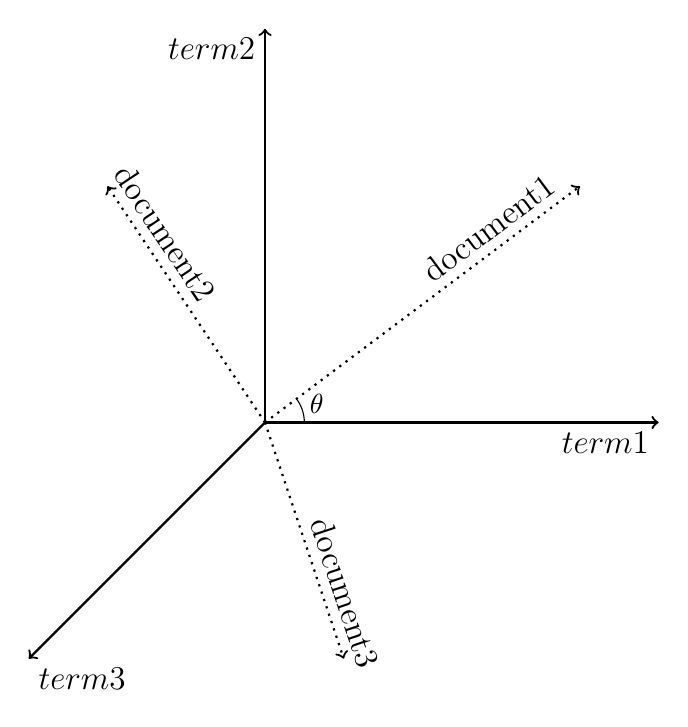
\begin{tikzpicture}
	
	%old version
	%\draw[->, thick] (0,0) -- (5,0);
	%\draw[->, thick] (0,0) -- (0,5);
	%\draw[->, thick] (0,0) -- (-3,-3);

	%\node at (5,-0.5) {\large term1};
	%\node at (-1,5) {\large term2};
	%\node at (-3.5,-3.5) {\large term3};

	%\draw[->, thick, dotted] (0,0) -- (4,3) node[near end, sloped,above] {\large document1};
	%\draw[->, thick, dotted] (0,0) -- (-2,3) node[near end, sloped,above] {\large document2};
	%\draw[->, thick, dotted] (0,0) -- (1,-3) node[near end, sloped,above] {\large document3};

	%axis
	\coordinate (o) at (0,0);
	\coordinate[label=below left: \large $term1$,] (x) at (5,0);
	\coordinate[label=below left:\large $term2$] (y) at (0,5);
	\coordinate[label=below right:\large $term3$] (z) at (-3,-3);

	\draw[->, thick] (o) -- (x);
	\draw[->, thick] (o) -- (y);
	\draw[->, thick] (o) -- (z);

	%vectors lines
	\coordinate (d1) at (4,3);
	\coordinate (d2) at (-2,3);
	\coordinate (d3) at (1,-3);

	\draw[->, thick, dotted] (o) -- (d1) node[near end, sloped,above] {\large document1};
	\draw[->, thick, dotted] (o) -- (d2) node[near end, sloped,above] {\large document2};
	\draw[->, thick, dotted] (o) -- (d3) node[near end, sloped,above] {\large document3};

	\begin{scope}
		\path[clip] (o) -- (d1) -- (x);
		\draw[draw = black] (o) circle (5mm);
		\node at ($(o)+(20:7mm)$) {$\theta$};
	\end{scope}
	


\end{tikzpicture}
\end{document}